\chapter{Indices d'immersion}
\par Nous allons maintenant présenter les différents indices de la catégorie <<~immersion~>>. Ces indices sont fournis par l'environnement immersif et ne participent pas à la vision directement ; ils sont généralement issus du mouvement de l'utilisateur. Pour ces critères, les valeurs clefs sont plus difficilement trouvables dans la littérature: on verra donc que, dans un premier temps, certains critères sont simplifiés et nécessiteraient un travail plus approfondi.
	
	\section{Latence}
	\par La latence peut avoir différentes définitions, que nous verrons plus en détails dans la partie consacrée entièrement à la latence. Néanmoins, on propose en première approche les définitions suivantes, pratiquées dans l'industrie:
	\begin{itemize}
		\item <<~Mouvement à photon~>>: depuis le mouvement effectué par un utilisateur jusqu'à l'affichage de ce mouvement dans la simulation (que ce soit un mouvement de la tête avec un calcul de point de vue, ou le mouvement d'une autre partie du corps, suivant ce qui est surveillé). Peut être simplifié comme la latence <<~totale~>> du système et est la définition généralement utilisée.
		\item <<~Mouvement à pré-calcul~>>: le temps écoulé entre un mouvement tracké et l'ordre de recalcul de l'image à une nouvelle position. Plus simplement, c'est le temps d'acquisition des capteurs de mouvements.
		\item <<~Pré-calcul à calcul~>>: temps écoulé pour générer le rendu visuel, par le traitement informatique de toutes les informations.
		\item <<~Calcul à photon~>>: temps écoulé entre la fin du calcul de rendu et la fin de l'affichage sur l'écran. C'est le temps qui s'écoule entre l'ordre d'actualisation de l'image et la fin de la modification de tous les pixels.
	\end{itemize}
	
	\par Bien qu'il existe des mesures de seuil de perception de la latence dans la littérature \citep{brooks_whats_1999,kemeny_driving_2014} et des valeurs de latence humaine pour les images claires (74~ms) et pour les images sombres (106~ms) \citep{feng_han_investigation_2010}, on souhaite compléter ces informations. On met donc sur pied une expérimentation pour étudier ce phénomène en comparant son influence dans la réalisation d'une tâche de visée dans un CAVE et dans un casque.
	
	\section{Champ de regard}
	\par Le champ de regard (FOR - Field of Regard en anglais) est l'extension du champ de vision: il est défini comme la portion d'espace qui est visible, au cours du temps, en incluant la possibilité de bouger la tête (mais pas le corps) et les yeux dans leurs orbites. De même que précédemment pour le champ de vision, on élabore une fonction de score divisée en deux branches; la branche horizontale (H-FOR) et la branche verticale (V-FOR). Ces deux axes sont ensuite pondérés l'un par rapport à l'autre.
	
	\subsection{Champ horizontal \& champ vertical}
	\par En prenant en compte les mouvements possibles de la tête et des yeux (jusqu'à 15 degrés), chaque œil peut couvrir un champ de regard de plus de 200 degrés du côté temporal et d'environ 130 degrés du côté nasal, sur l'axe horizontal. L'axe vertical représente lui environ 310 degrés répartis à +140 et -170 d'après \citep{fuchs_traite_2003}.
	
	\par D'un côté, et parce que le champ visuel se recouvre, on limite la valeur maximale de H-FOR à 360 degrés ($h_{max}$). Le maximum de V-FOR est lui laissé tel quel à 310 degrés ($v_{max}$). De l'autre côté, les valeurs minimales ne peuvent pas être plus petites que les valeurs mesurées pour le champ de vision. On les nomme ici $h_0$ et $v_0$ mais ont les même valeurs que les $h$ et $v$ du champ de vision. L'évolution de la notation est linéaire pour chaque axe entre le minimum et le maximum.
	
	\par L'équation est donc (Eq. \ref{eq:field_of_regard_sub_items}), pour le champ de regard horizontal (H-FOR) et (V-FOR), avec $h$ et $v$ les valeurs mesurées des axes horizontaux et verticaux ; et $h_{0}$, $v_{0}$, $h_{max}$, $v_{max}$ défini précédemment pour le champ de vision:
	\begin{equation}
	\begin{cases}
		F_{H-FOR}(h) = \frac{100}{h_{max} - h_0} \cdot (h - h_0)\\
		F_{V-FOR}(v) = \frac{100}{v_{max} - v_0} \cdot (v - v_0)
	\end{cases}
	\label{eq:field_of_regard_sub_items}
	\end{equation}
	
	\subsection{Pondération}
	\par En faisant la même hypothèse que pour la pondération du champ de vision, on base les poids relatifs des deux axes sur leurs tailles respectives: 400 degrés pour l'axe horizontal et 310 pour l'axe vertical. Les 400 degrés de l'axe horizontal diffèrent des 360 utilisés pour la notation de l'axe (pour laquelle on avait limité l'angle à 360 degrés) et peuvent interpeller. Si mécaniquement lorsque que l'on regarde autour de soi on regarde à 360 degrés, dans les faits comme les demi-champs de regard (celui du côté temporal et celui du côté nasal) sont supérieurs à 180 degrés, on peut voir une petite partie de l'autre demi-champ de regard: une partie de l'espace est visible de deux manières (voir Fig. \ref{fig:demi_champs_regard}). En terme de possibilités donc le champ est plus grand que 360 degrés d'où la valeur de 400 degrés conservée. On utilise donc la même méthodologie que pour le champ de vision et on obtient (Eq. \ref{eq:field_of_regard_weighting}):
	\begin{equation}
	\begin{cases}
		k_h = \frac{400}{400 + 310} = 0.56\\
		k_v = 1 - k_h = 0.44
	\end{cases}
	\label{eq:field_of_regard_weighting}
	\end{equation}
	
	\begin{figure}[h]
		\centering
		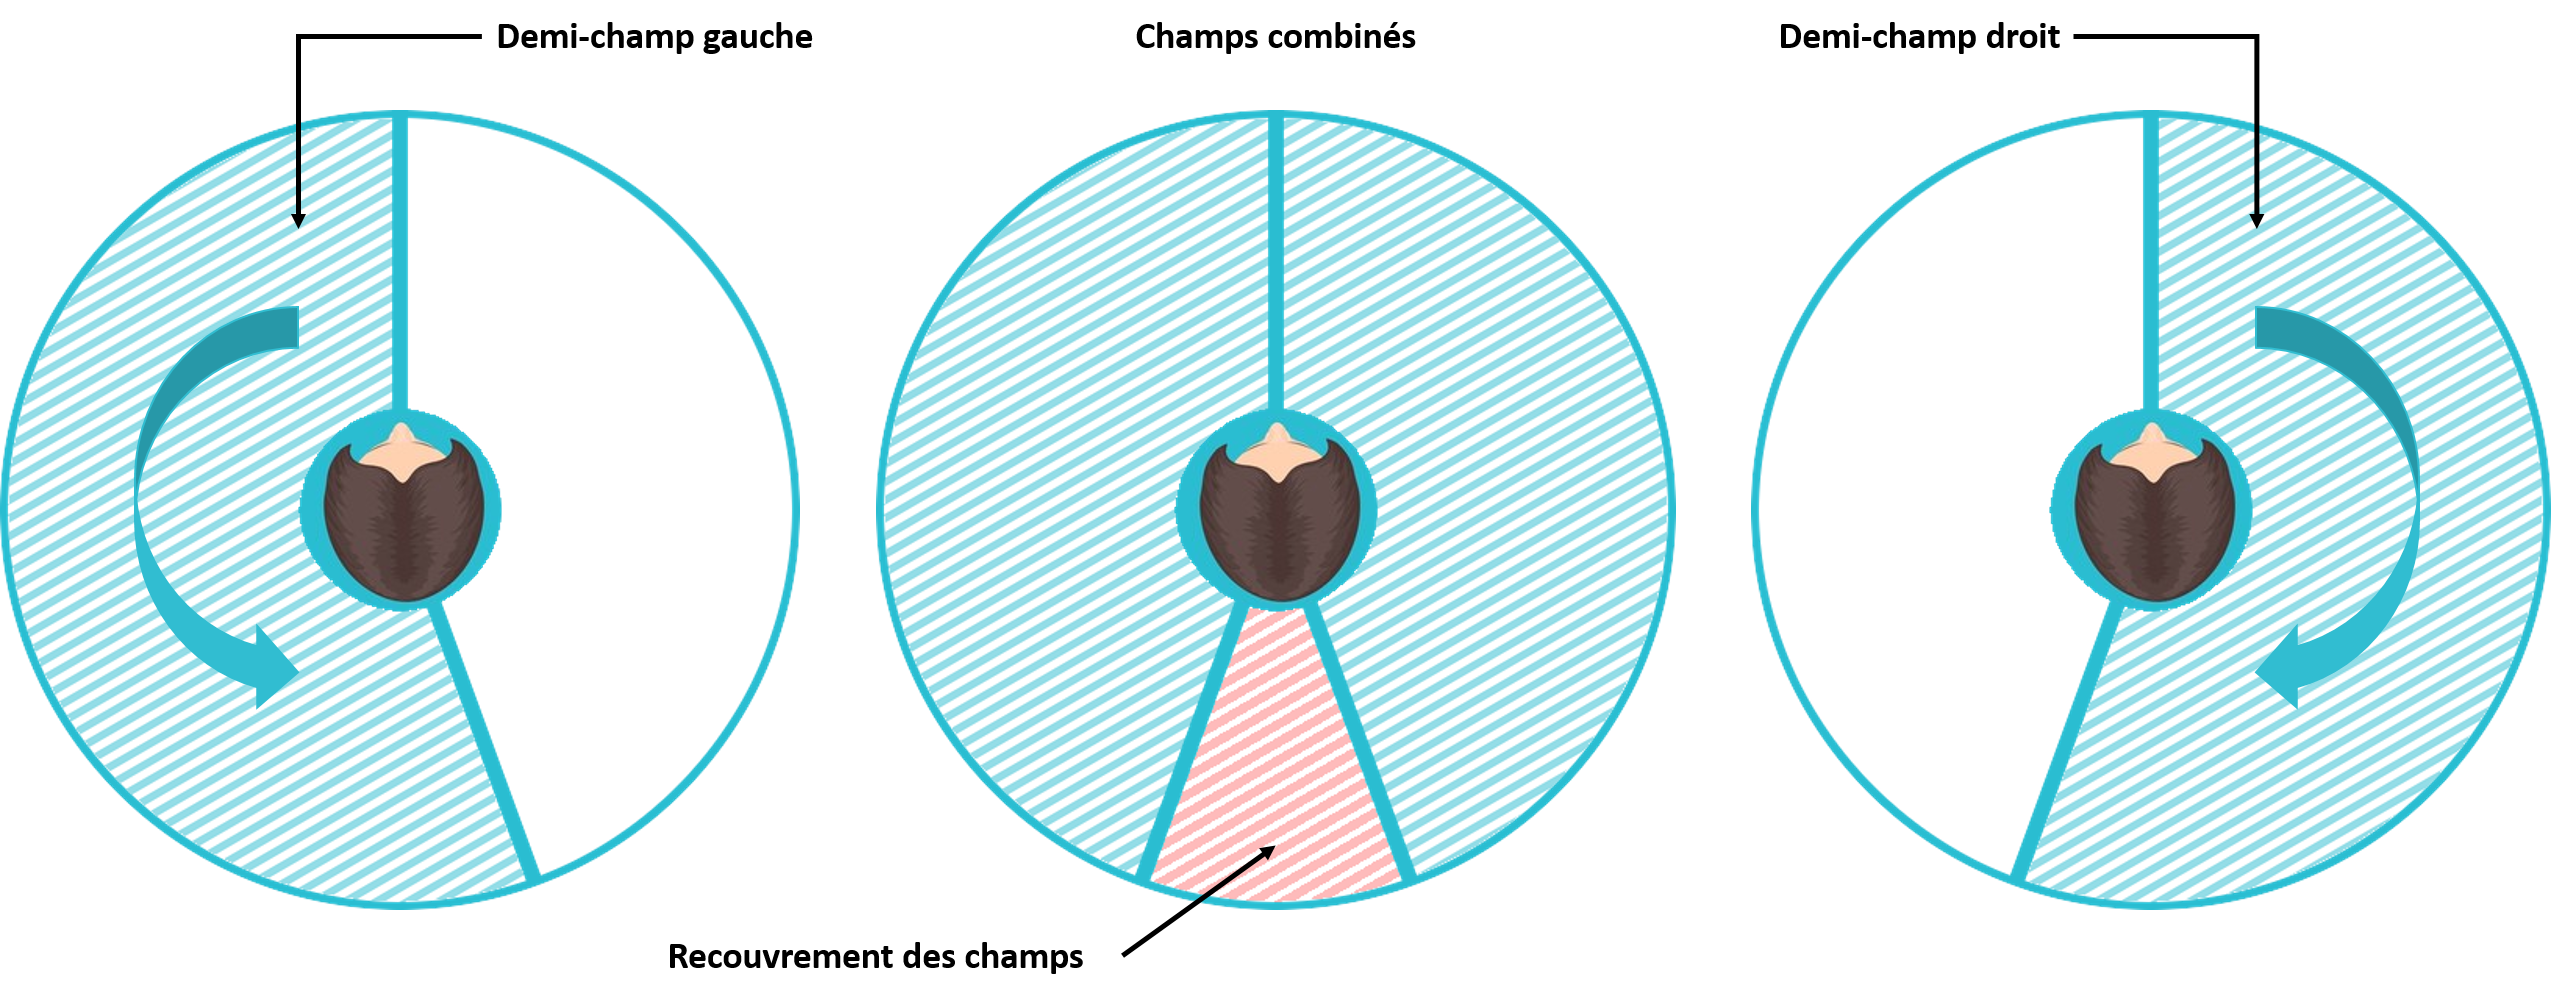
\includegraphics[scale=.35]{Figures/RecouvrementFOR}
		\caption{Recouvrement des demi-champs de regard (temporal et nasal).}
		\label{fig:demi_champs_regard}
	\end{figure}
	
	\par Ce qui est finalement assez proche de la pondération du champ de vision. Au final, la fonction de notation du champ de regard est définie par l'équation suivante (Eq. \ref{eq:score_field_of_regard}):
	\begin{equation}
	F_{FOR}(h,v) = k_h \cdot F_{H-FOR}(h) + k_v \cdot F_{V-FOR}(v)
	\label{eq:score_field_of_regard}
	\end{equation}
	
	\par Cette hypothèse de pondération est valable pour le cas général. On a vu par la suite, qu'elle pouvait être mise à mal dans certains cas de figures (voir chapitre sur l'expérimentation comparative entre les scores d'acceptation et les scores du modèle) et qu'il fallait, dans le cas par exemple d'une simulation de conduite, mettre la quasi intégralité de la pondération sur le champ de regard horizontal.
	
	\section{Stéréoscopie}
	\subsection{Fonctionnement}	
	\par La stéréoscopie est une méthode pour donner de la profondeur et du relief à des images  standard en 2D. Les yeux, de part leur écartement, ont des images d'un point de vue toujours différent. En combinant les informations (et notamment les différences entre les deux points de vue) le cerveau est capable de récréer la profondeur. Le principe de la stéréoscopie est donc de fournir à chaque œil une image différente, calculée avec le bon point de vue. Cela peut être réalisé via un certain nombre de techniques \citep{mehrabi_making_2013}. On se concentre dans notre cas sur les méthodes avec des lunettes portées (Casque, lunettes obturantes, lunettes polarisées, anaglyphes, ...). Ces dernières sont présentées par \cite{fauster_stereoscopic_2007}. On rappelle ici les deux techniques les plus connues (historiquement) pour amener du relief.
	
	\par Le type de stéréoscopie le plus connu du grand public est surement la technique dite <<~anaglyphe~>> qui fonctionne avec des lunettes aux verres rouge et bleu (voir Fig. \ref{fig:stereo_glasses}). Le principe est d'afficher les deux images nécessaires à la stéréoscopie en même temps mais chacune superposée par un filtre de couleur rouge ou de couleur bleue. Le verre rouge ne laisse passer que l'image rouge tandis que le filtre bleu ne laisse passer que son image de couleur correspondante. Chaque œil voit donc une seule image et le cerveau peut ainsi reconstruire la profondeur.
	
	\begin{figure}[h]
		\centering
		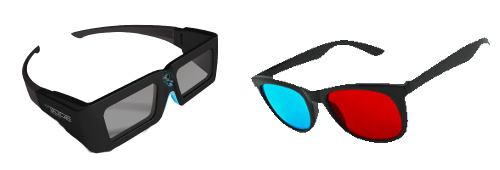
\includegraphics[scale=.8]{Figures/StereoActiveAnaglyphGlasses}
		\caption{Lunettes de stéréoscopie.}
		\label{fig:stereo_glasses}
	\end{figure}
	
	\par L'autre technique répandue est la stéréo dite <<~active~>> ; c'est celle utilisée par exemple dans les cinémas, mais surtout pour le cas qui nous intéresse, dans l'industrie. Cette fois, les lunettes ont des filtres identiques et relativement transparents (voir Fig. \ref{fig:stereo_glasses}). Les images destinées aux yeux sont affichées l'une après l'autre (et pas en même temps comme la technique précédente) et ce sont les lunettes qui font le tri pour attribuer la bonne image au bon œil: de manière synchronisée avec l'affichage des images un verre devient opaque tandis que l'autre est transparent et ainsi de suite en alternance. Lorsque l'image pour l'œil gauche est affichée, le verre gauche laisse passer la lumière quand le verre droit la bloque, et inversement.
	
	\par Il existe aussi d'autres moyens de recréer une vision binoculaire comme les affichages auto-stéréoscopiques ou les affichages holographiques mais qui sortent du cadre d'étude car on se concentre sur les simulateur immersifs basés sur des techniques de stéréoscopie active. 
	
	\subsection{Fonction de notation du critère}
	\par En première approche, qui serait à étoffer, on propose de noter le critère sur sa présence (100) ou son absence (0). La piste d'amélioration à suivre pourrait être une découpe de la fonction de notation par rapport à la technique utilisée: toutes les techniques ne se valent pas et leurs performances pourraient être comparées. Il ne semble pas encore y avoir de telle comparaison dans la littérature. On propose en Fig. \ref{fig:stereo_grade_techno} un exemple à titre d'illustration uniquement.
	
	\begin{figure}[h]
		\centering
		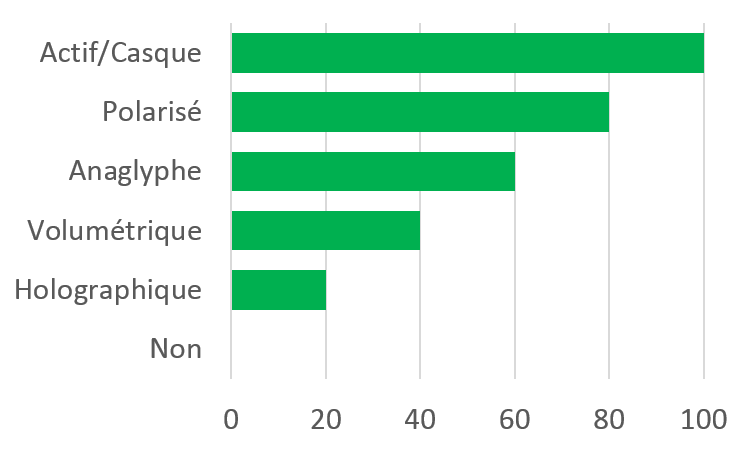
\includegraphics[scale=1]{Figures/StereoTechnoScore}
		\caption{Illustration d'une notation du critère <<~Stéréoscopie~>> en fonction de la technologie}
		\label{fig:stereo_grade_techno}
	\end{figure}
	
	\section{Tracking}
	\par Le tracking est surement un des éléments les plus importants pour l'immersion. Le tracking permet d'inclure les mouvements de l'utilisateur dans la simulation, que ce soit du corps ou de la tête, mais aussi l'inclusion d'appareils extérieurs ou autres. Là encore, il existe un grand nombre de techniques, que ce soit embarqué dans les casque de réalité virtuelle ou bien avec des solutions externes. Dans le cas d'un CAVE on utilise en général des caméras infrarouge et un système de boules réfléchissantes sur les objets (ou parties du corps) à repérer dans l'espace (voir Fig. \ref{fig:tracking_illustration}). Pour chaque objet dont on souhaite connaitre la position dans l'espace, on fixe au minimum trois boules réfléchissant les rayons infrarouges. Ces trois boules doivent être en permanence au même endroit sur l'objet et dans la même configuration (voir Fig. \ref{fig:tracking_illustration}, des deux côtés des lunettes). On balaye ensuite l'espace à tracker avec des caméras émettant et captant les rayons infrarouges. Le système de boules réfléchit ces rayons et est ainsi vu par les différentes caméras qui, comme elles sont placées à différents endroits dans l'espace, peuvent trianguler la position et l'orientation de l'objet étant donné que les boules réfléchissantes sont fixes par rapport à l'objet.
	
	\begin{figure}[h]
		\centering
		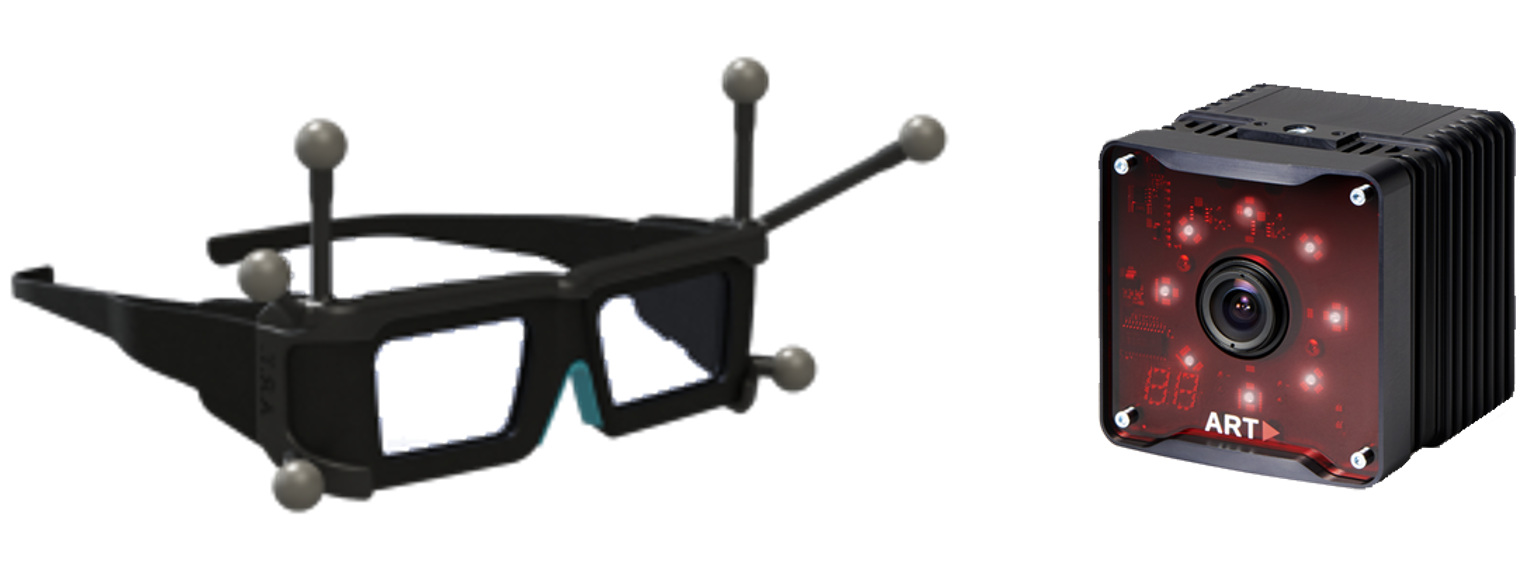
\includegraphics[scale=.6]{Figures/TrackingCameraBody}
		\caption{<<~Body~>> de tracking monté sur des lunettes de stéréoscopie \& ensemble caméra-émetteur infrarouge pour le tracking.}
		\label{fig:tracking_illustration}
	\end{figure}
	
	\par A défaut, et en attendant, de proposer une notation sur des critères plus développés, on propose de noter simplement ce critère sur sa présence (100) ou son absence (0). L'élément à creuser serait sa précision, c'est à dire son écart de position entre la position réelle de l'objet/body de tracking et la position vue par le système. Cette précision dépend néanmoins d'autres paramètres comme la calibration des caméras ou la calibration de la <<~room~>> (la définition des bordures de l'espace de travail). Il pourrait être aussi envisageable, au même titre que pour la stéréoscopie, de traiter le tracking en fonction de la technologie. Il faudrait alors comparer le tracking infrarouge avec le tracking magnétique ou autre.
		
	\section{Uniformité}
	\par Bien que défini dans le modèle, le critère d'uniformité est le seul qui n'a pas été pleinement abordé. C'est un sujet complexe qui se divise en plusieurs partie. L'uniformité peut à la fois valoir à l'intérieur d'un même écran, c'est à dire entre différentes zones d'un écran, mais aussi -quand le système le permet de part sa construction- entre les différents écrans. Même si l'uniformité la plus évidente concerne la couleur (on souhaite qu'un rouge affiché soit identique partout), il faut en fait l'élargir au d'autres critères:
	\begin{itemize}
		\item la couleur,
		\item la luminosité,
		\item le contraste.
	\end{itemize}
	
	\par La couleur est surement le critère le plus facile à vérifier car on sait mesurer des écarts entre les couleurs grâce aux équations de différentiations des couleurs (présentées dans la première partie du manuscrit). Ces équations donnent donc des écarts entre les couleurs qui, par construction doivent être inférieurs à une valeur de 1 pour qu'ils soient imperceptibles à l'oeil humain. Néanmoins, en informatique notamment, le seuil réel est plus bas (la valeur en dessous de laquelle la différence est imperceptible est plus grand que le 1 théorique) pour les population experte dans le domaine de la couleur, et encore plus bas pour les populations néophytes \citep{vidal_color-difference_2016}. On pourrait donc se baser sur ces trois valeurs (valeur théorique minimale, valeur de la population experte et valeur de la population néophyte) pour faire une première échelle de notation.
	
	\par Néanmoins, on présente ici les valeurs qui sont utilisées dans les cahiers des charges de Renault pour le design des moyens immersifs du groupe. Ces valeurs sont le fruit de l'expérience des ingénieurs et d'échanges avec les différents acteurs du milieu. Toutes les mesures sont faites selon la norme ANSI IT7.215, c'est à dire avec 9 points de mesure sur chaque écran. Ces points sont répartis en 3 lignes de 3: sur chaque ligne, un point centré encadré par deux autres points distants de 1/3 de la largeur totale de l'écran par rapport au bord.
	
	\par Pour la couleur, le mesures se font indépendamment sur du blanc uni et un gris 18\% uni (Gris RGB 128). Les spécifications sont à appliquer à la fois entre les différents points de mesure sur l'écran mais également entre les écrans, lorsque c'est le cas dans le système immersif. Dans le premier cas, le $\Delta E$ maximal toléré est de 6. Dans le deuxième cas, pour deux faces contiguës, seuls les 3 points les plus proches des bords en contact sont concernés. Un $\Delta E$ maximal de 6 est également requis.
	
	\par Pour la luminance, la différence entre le point le plus lumineux et le point le plus sombre ne doit pas dépasser 30\%, sur la base de la plus petite valeur mesurée. En cas d'écrans contigus, la différence entre le point le plus lumineux et le point le plus sombre ne doit pas dépasser 10\%, là encore sur la base de la plus petite valeur mesurée. De manière analogue aux spécifications sur la couleur, on n'utilise pas les 18 points de mesure mais seulement les 6 points les plus proches des bords comparés (3 par écran).
	
	\par Pour le contraste, la différence entre la valeur minimale et et la valeur maximale entre les différents écrans ne doit pas dépasser 25\% de la valeur minimale.
	
	\section{Orientation des caméras}	
	\subsection{Mimétisme du fonctionnement oculaire}	
	\par La capture d'image dans une scène virtuelle pour affichage sur un/des écran-s se fait au moyen d'une <<~caméra~>> virtuelle. Dans le cas de la stéréoscopie, comme il est nécessaire d'avoir une image par œil, deux caméras virtuelles entrent en jeu. Ces caméras sont l'équivalent virtuel de nos yeux. Il semblerait donc naturel que les caméras aient un comportement relativement proche de ces derniers et pourtant ce n'est majoritairement pas le cas.
	
	\par Lorsque l'on regarde un objet proche de nous, les yeux s'orientent dans leur orbite et se tournent vers cet objet. Plus l'objet est proche, plus il est nécessaire de converger. Au contraire, quand l'objet recule, et à partir d'une certaine distance, celui-ci est considéré comme <<~à l'infini~>> et les directions des yeux sont parallèles, soit avec une convergence nulle. Dans la majeure partie des cas, la convergence des caméras n'est pas implémentée: on parle alors de caméras <<~parallèles~>> (ou à <<~convergence~>> nulle). La raison vient du fait qu'utiliser des caméras arbitrairement convergées (et qui resteraient convergées, donc à <<~convergence fixe~>>) entraine automatiquement un certain nombre de distorsions \citep{woods_image_1993}. Si l'utilisateur regarde un objet à une <<~convergence~>> différente de celle qui est prévue, l'orientation des caméras n'est pas la bonne. Ainsi, plutôt par soucis de simplicité, on fait en général l'hypothèse que tous les objets (ou en tout cas la majorité) seront suffisamment éloignés pour être dans une situation de convergence nulle.
	
	\par Néanmoins on peut optimiser l'utilisation de ces distorsions si l'on est capable de régler la convergence des caméras en temps réel en fonction de la distance à laquelle l'utilisateur regarde. Cet ajout s'avère même bénéfique car il ajoute des disparités verticales qui font partie du processus de vision \citep{aurat_immersion_2016}. On peut alors parler de <<~caméras à convergence variable~>>. Il faut alors acquérir la position du regard en temps réel, ce qui peut être fait soit matériellement en ajoutant par exemple un système de tracking du regard (voir Fig. \ref{fig:eye_tracker}), soit en faisant des hypothèses telles que la personne regarde droit devant elle (et non en coin), donc la direction du regard est la même que la direction de la tête. La mise en œuvre de la convergence n'est également pas facilitée par le fait de capturer des images dans des plans non parallèles au plan de projection final. Les caméras convergées capturent des images planes mais dans un plan qui ne correspond par forcément à la surface sur laquelle il faudra la projeter (voir Fig. \ref{fig:redressement_plan_vision}). Il faut donc passer par une étape supplémentaire de warping de l'image \citep{aurat_immersion_2016}.
	
	\begin{figure}[h]
		\centering
		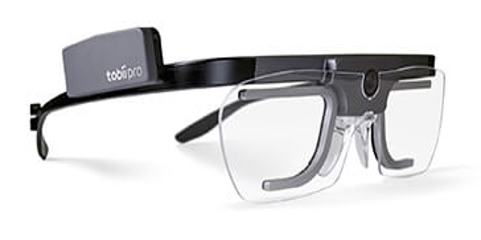
\includegraphics[scale=1]{Figures/EyeTrackerTobii}
		\caption{Exemple de système de tracking de regard portatif.}
		\label{fig:eye_tracker}
	\end{figure}
	
	\begin{figure}[h]
		\centering
		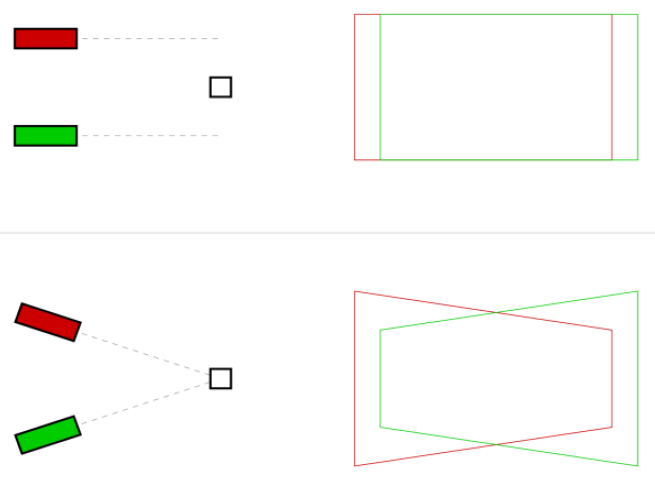
\includegraphics[scale=.75]{Figures/RedressementPlansVision}
		\caption{Exemple de déformation due à la convergence des caméras.}{Le carré est vu comme deux rectangles dans une configuration <<~caméras à convergence nulle~>> et comme deux trapèzes lorsque les caméras sont convergentes. Il faut donc retordre artificiellement les trapèzes pour qu'ils correspondent à la projection qui se fait sur une surface rectangulaire (image tirée de \citep{aurat_immersion_2016}).}
		\label{fig:redressement_plan_vision}
	\end{figure}
	
	\par Cette dichotomie entre la convergence réelle des yeux et la convergence artificielle des caméras virtuelles n'est pas anodine car elle est à l'origine d'un des plus grand maux dans les simulateurs: le conflit accommodation-vergence qui génère notamment des fatigues, fatigues visuelles, participe au mal du simulateur et dégrade grandement la qualité d'immersion \citep{neveu_impact_2012}. En effet, les images sont affichées sur un écran à une certaine distance auquel les yeux s'accommodent tandis que les images jaillissent (ou inversement, s'enfoncent) de l'écran, obligeant les yeux à converger dessus. L'accommodation et la convergence qui sont normalement liées sont dès lors désynchronisées et génèrent un conflit pour le cerveau.
	
	\subsection{Fonction de notation du critère}
	\par Ainsi, le critère est divisé en trois, soit le nombre de possibilité qui existent:
	\begin{itemize}
		\item caméras à convergence fixe (c'est à dire sans connaitre le point de regard), 0.
		\item caméras à convergence nulle (caméras parallèles), 80.
		\item caméras à convergence variable (avec connaissance du point de regard), 100.
	\end{itemize}